\documentclass[a4paper,12pt]{article} 



%Добавляет возможность искать и копировать текст
\usepackage{cmap}

%Убирает пробел между названием таблицы/рисунка и самой таблицей/рисунком
\usepackage{caption}
\captionsetup[table]{skip= -0 cm}
\captionsetup[figure]{skip= -0 cm}

%Выравнивание названия таблиц по левому краю
%\usepackage[nooneline]{caption} 
%Размеры отступов 
\usepackage[left=20mm, top=20mm, right=20mm, bottom=20mm, footskip=10mm]{geometry}

%Рисунки
\usepackage{graphicx}
\usepackage{wrapfig} %обтекание элементов
\graphicspath{{graphs}{figures}}  % папки с картинками

%Русский язык в формулах
\usepackage{mathtext}

%  Русский язык
\usepackage[T2A]{fontenc}			
\usepackage[utf8]{inputenc}			
\usepackage[english,russian]{babel}	

%Готические буквы
\usepackage{amssymb}

% Математика
\usepackage{amsmath,amsfonts,amssymb,amsthm,mathtools} 
\usepackage{wasysym}

%Цветные подписи в таблице
\usepackage[table,xcdraw]{xcolor}

\usepackage{fancyhdr} % Колонтитулы
 	\pagestyle{fancy}
 	\renewcommand{\headrulewidth}{0.3mm}  % Толщина линейки, отчеркивающей верхний колонтитул
 	%\lfoot{Нижний левый}
 	%\rfoot{Нижний правый}
 	\rhead{Кафедра вакуумной электроники}
 	%\chead{Верхний в центре}
 	\lhead{Электронно-оптический преобразователь}
 	% \cfoot{Нижний в центре} % По умолчанию здесь номер страницы
 	
 	
\begin{document} 

%Титульник 
\begin{titlepage}
	\begin{center}
		\large 	МИНИСТЕРСТВО ОБРАЗОВАНИЯ И НАУКИ РОССИЙСКОЙ ФЕДЕРАЦИИ\\
				МОСКОВСКИЙ ФИЗИКО-ТЕХНИЧЕСКИЙ ИНСТИТУТ \\
				(НАЦИОНАЛЬНЫЙ ИССЛЕДОВАТЕЛЬСКИЙ ИНСТИТУТ)\\ 
				ФИЗТЕХ-ШКОЛА ЭЛЕКТРОНИКИ, ФОТОНИКИ \\
				И МОЛЕКУЛЯРНОЙ ФИЗИКИ \\
		
		
		\vspace{4.0 cm}
		\LARGE{Кафедра вакуумной электроники \\ 
		Отчет \\
		по лабораторной работе} \\ 
		\LARGE \textbf{Электронно-оптический преобразователь} \\

	\end{center}
	\vspace{3 cm} \large

	%Надо подумать как это нормально написать	
	\begin{flushleft}
		Работу выполнили \hspace{0.5cm}  \underline{\hspace{3cm}} Белостоцкий, Вовк Алешин, Мусатов \\	
		\vspace{1cm}
		Работу принял, оценка \hspace{0cm} \underline{\hspace{3cm}}
	\end{flushleft}

	
	\vfill

	\begin{center}
	Долгопрудный, 2021 г.
	\end{center}
\end{titlepage}                                                                      

\section*{Цель работы} 
\begin{itemize}
\item Ознакомиться с принципами работы электронно-оптического преобразователя
\end{itemize}

\section*{Теоретические сведения} 	

Электронно-оптические преобразователи (ЭОП) – это вакуумные приборы, сначала преобразующие оптическое изображение в электронный аналог, т.е. в электронное изображение, которым можно эффективно управлять электрическим полем (усиливать, отклонять по координате и т.д.), после чего оно проецируется на люминесцентный экран, где снова преобразуется в оптическое изображение. 

ЭОП представляет собой электровакуумную колбу, внутри которой размещены фотокатод, люминесцентный экран,  фокусирующая и ускоряющая электронно-оптические системы. В ЭОП, используемом в лабораторной работе для усиления электрического тока применяется микроканальная пластина.

\begin{figure}[h!]
	\begin{center}
	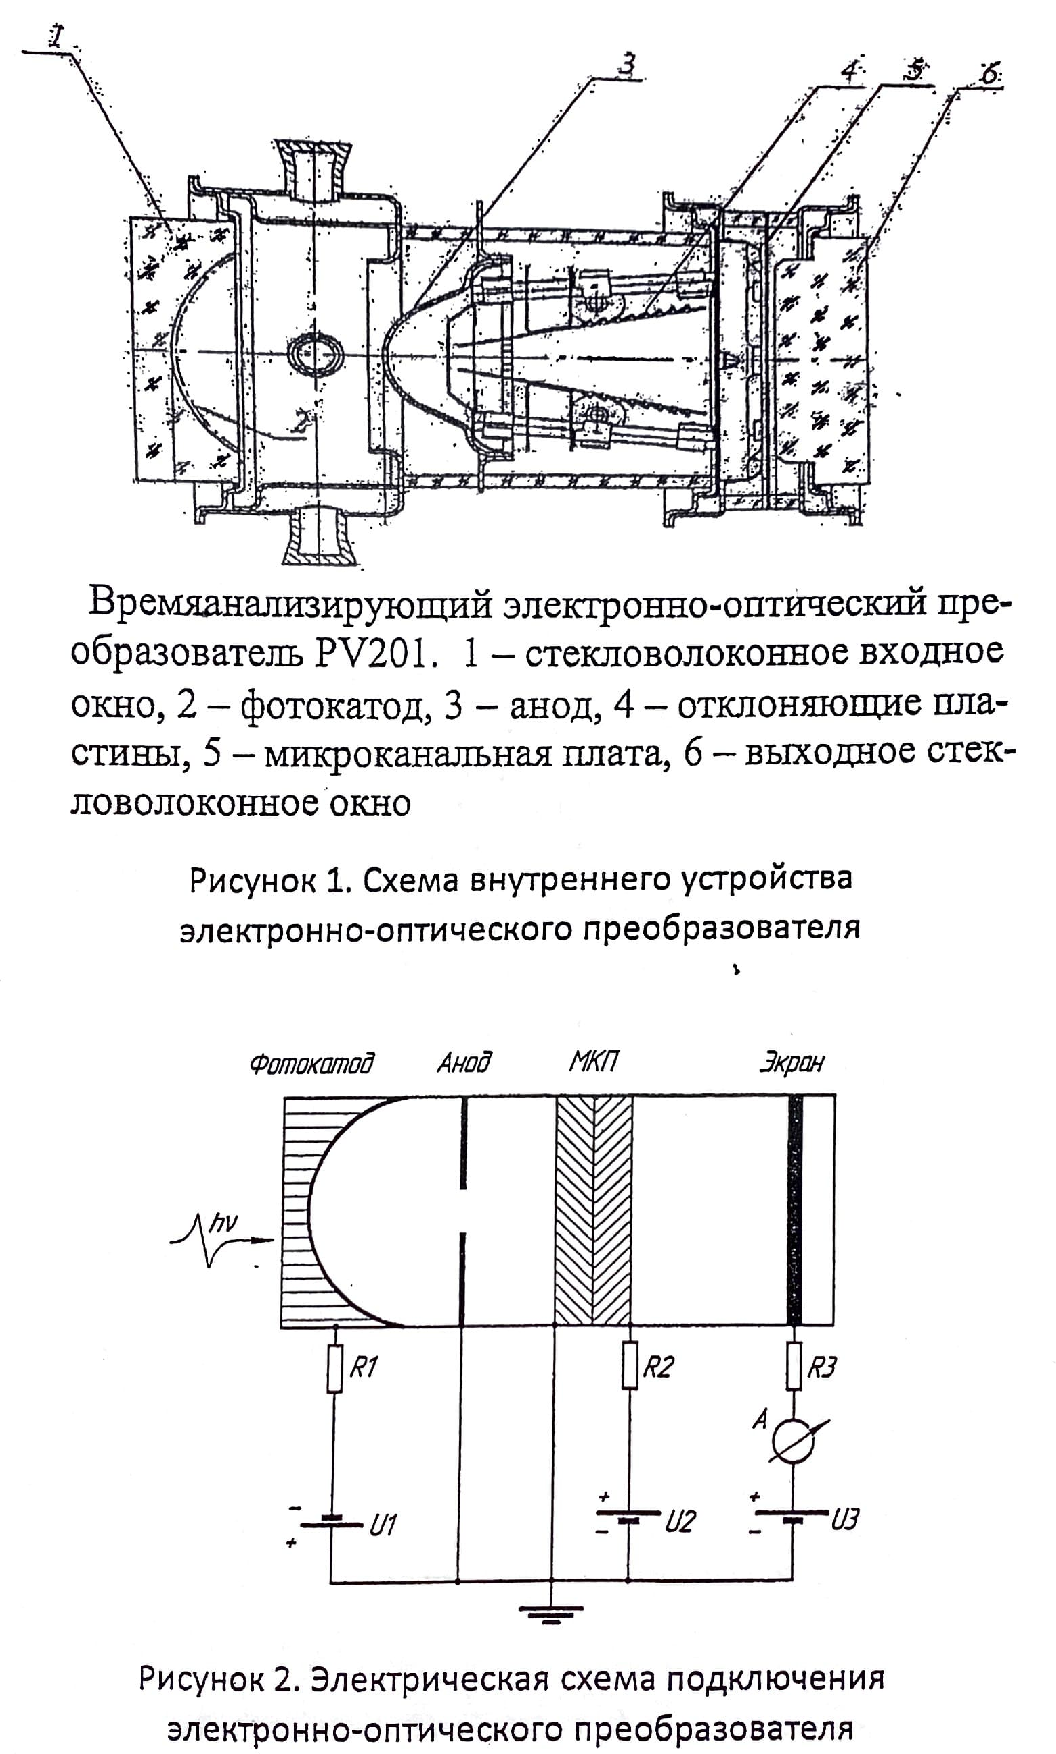
\includegraphics[scale=0.4]{fig1}
	\end{center}
\end{figure}

Когда налетающий электрон попадает в канал, то из стенки канала выбиваются вторичные электроны, которые ускоряются электрическим полем вдоль канала. Электрическое поле внутри канала создаётся путём приложения напряжения между поверхностями МКП (концами каналов). Вторичные электроны летят, пока не попаут на стенку, в свою очередь выбивая ещё большее количество вторичных электронов. Этот процесс по мере пролёта вдоль канала повторяется много раз, и на выходе канала формируется электронная лавина.

\section*{Ход работы}

Приводим установку в рабочее состояние. При помощи ручек мы имеем возможность регулировать напряжение катода, напряжение экрана и напряжение МКП и регистрировать ток анода, катода, МКП и экрана. По умолчанию значения напряжений МКП, экрана и катода равны 3 кВ, 2 кВ и 3 кВ соответственно

При значениях напряжения на экране и МКП по умолчанию меняем напряжение на катоде и фиксируем значения всех токов. Полученные данные занесем в Таблицу $\ref{table:katod}$

\begin{table}[h]
\begin{center}
\caption{Зависимости токов от напряжения на катоде}
\label{table:katod}
\begin{tabular}{|ccccc|}
\hline
\multicolumn{1}{|c|}{\textbf{U}, кВ} & \multicolumn{1}{c|}{\textbf{$I_{катод}$}, мкА} & \multicolumn{1}{c|}{\textbf{$I_{МКП}$}, мкА} & \multicolumn{1}{c|}{\textbf{$I_{экран}$}, мкА} & {\textbf{$I_{анод}$}, мкА} \\ \hline
\multicolumn{1}{|c|}{0,9}            & \multicolumn{1}{c|}{0}                      & \multicolumn{1}{c|}{8,84}            & \multicolumn{1}{c|}{0}                 & 4,46             \\ \hline
\multicolumn{1}{|c|}{1,25}           & \multicolumn{1}{c|}{0,01}                   & \multicolumn{1}{c|}{8,82}            & \multicolumn{1}{c|}{0}                 & 4,47             \\ \hline
\multicolumn{1}{|c|}{1,55}           & \multicolumn{1}{c|}{0}                      & \multicolumn{1}{c|}{8,82}            & \multicolumn{1}{c|}{0}                 & 4,46             \\ \hline
\multicolumn{1}{|c|}{1,81}           & \multicolumn{1}{c|}{0}                      & \multicolumn{1}{c|}{8,84}            & \multicolumn{1}{c|}{0}                 & 4,46             \\ \hline
\multicolumn{1}{|c|}{2,16}           & \multicolumn{1}{c|}{0}                      & \multicolumn{1}{c|}{8,84}            & \multicolumn{1}{c|}{0}                 & 4,48             \\ \hline
\multicolumn{1}{|c|}{2,5}            & \multicolumn{1}{c|}{0,02}                   & \multicolumn{1}{c|}{8,82}            & \multicolumn{1}{c|}{0,05}              & 4,48             \\ \hline
\multicolumn{1}{|c|}{2,74}           & \multicolumn{1}{c|}{0}                      & \multicolumn{1}{c|}{8,82}            & \multicolumn{1}{c|}{0,07}              & 4,5              \\ \hline
\multicolumn{1}{|c|}{3,14}           & \multicolumn{1}{c|}{0}                      & \multicolumn{1}{c|}{8,82}            & \multicolumn{1}{c|}{0,09}              & 4,51             \\ \hline
\multicolumn{1}{|c|}{3,65}           & \multicolumn{1}{c|}{0,02}                   & \multicolumn{1}{c|}{8,84}            & \multicolumn{1}{c|}{0,1}               & 4,52             \\ \hline
\multicolumn{1}{|c|}{4,03}           & \multicolumn{1}{c|}{0}                      & \multicolumn{1}{c|}{8,84}            & \multicolumn{1}{c|}{0,12}              & 4,53             \\ \hline
\multicolumn{1}{|c|}{4,26}           & \multicolumn{1}{c|}{0}                      & \multicolumn{1}{c|}{8,84}            & \multicolumn{1}{c|}{0,11}              & 4,53             \\ \hline
\end{tabular}
\end{center}
\end{table}

По данным Таблицы $\ref{table:katod}$ построим графики зависимостей токов от напряжения на катоде


\begin{figure}[h!]
	\begin{center}
	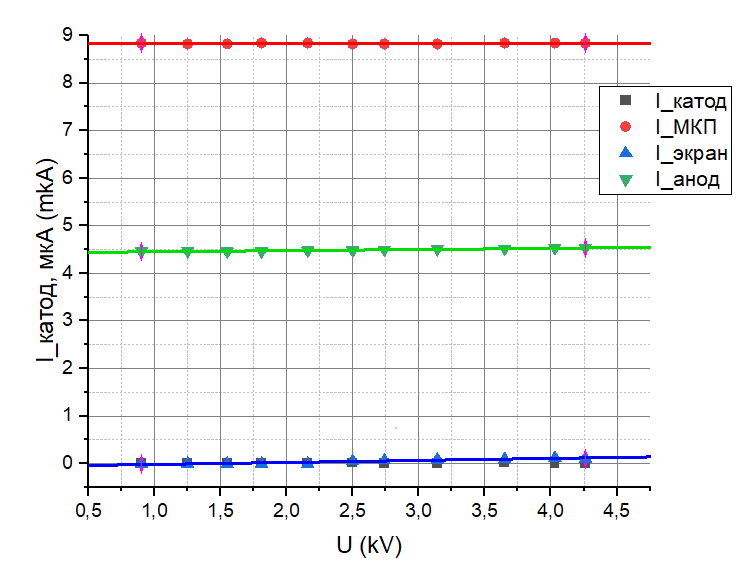
\includegraphics[scale=0.8]{1}
	\label{graph:katod}
	\caption{Зависимость токов от напряжения на катоде}
	\end{center}
\end{figure}

\newpage

При значениях напряжения на экране и катоде по умолчанию меняем напряжение на МКП и фиксируем значения всех токов. Полученные данные занесем в Таблицу $\ref{table:MKP}$

\begin{table}[h]
\begin{center}
\caption{Зависимость токов от напряжения на МКП}
\label{table:MKP}
\begin{tabular}{|c|c|c|c|c|}
\hline
{\textbf{U}, кВ} & \multicolumn{1}{c|}{\textbf{$I_{катод}$}, мкА} & \multicolumn{1}{c|}{\textbf{$I_{МКП}$}, мкА} & \multicolumn{1}{c|}{\textbf{$I_{экран}$}, мкА} & {\textbf{$I_{анод}$}, мкА}  \\ \hline
0,32       & 0                 & 1,34            & 0                 & 0,66             \\ \hline
0,56       & 0                 & 2,3             & 0                 & 1,13             \\ \hline
0,75       & 0                 & 3,1             & 0                 & 1,56             \\ \hline
1          & 0                 & 4,18            & 0                 & 2,1              \\ \hline
1,39       & 0                 & 5,89            & 0                 & 2,97             \\ \hline
1,72       & 0                 & 7,45            & 0                 & 3,77             \\ \hline
2          & 0                 & 8,76            & 0,08              & 4,48             
\\ \hline
\end{tabular}
\end{center}
\end{table}

По данным Таблицы $\ref{table:MKP}$ построим графики зависимостей токов от напряжения на МКП

\begin{figure}[h!]
	\begin{center}
	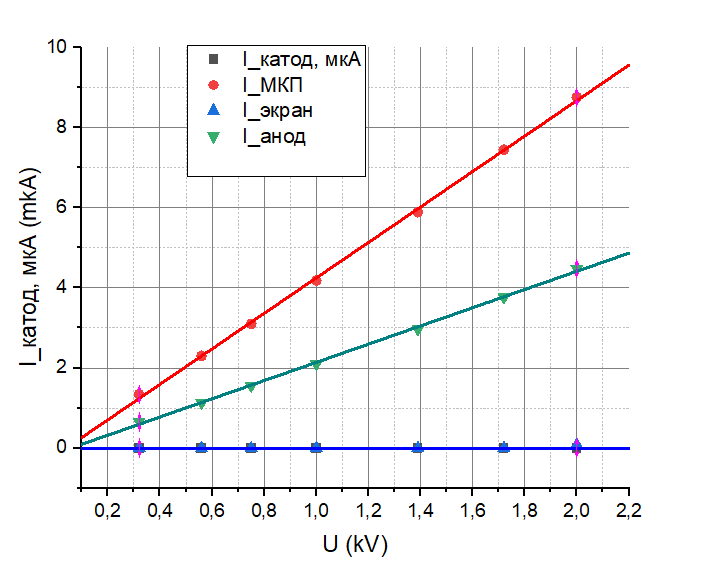
\includegraphics[scale=1]{2}
	\label{graph:MKP}
	\caption{Зависимость токов от напряжения на МКП}
	\end{center}
\end{figure}

\newpage

При значениях напряжения на экране и катоде по умолчанию меняем напряжение на МКП и фиксируем значения всех токов. Полученные данные занесем в Таблицу $\ref{table:ekran}$

\begin{table}[h]
\begin{center}
\caption{Зависимость токов от напряжения на экране}
\label{table:ekran}
\begin{tabular}{|c|c|c|c|c|}
\hline
{\textbf{U}, кВ} & \multicolumn{1}{c|}{\textbf{$I_{катод}$}, мкА} & \multicolumn{1}{c|}{\textbf{$I_{МКП}$}, мкА} & \multicolumn{1}{c|}{\textbf{$I_{экран}$}, мкА} & {\textbf{$I_{анод}$}, мкА} \\ \hline
0,82       & 0                 & 8,8             & 0,06              & 4,48             \\ \hline
1,13       & 0                 & 8,8             & 0,07              & 4,49             \\ \hline
1,52       & 0                 & 8,8             & 0,06              & 4,49             \\ \hline
1,85       & 0                 & 8,8             & 0,06              & 4,49             \\ \hline
2,12       & 0                 & 8,8             & 0,06              & 4,49             \\ \hline
2,5        & 0                 & 8,8             & 0,06              & 4,49             \\ \hline
2,81       & 0                 & 8,8             & 0,06              & 4,49             \\ \hline
3,09       & 0                 & 8,8             & 0,06              & 4,49             \\ \hline
3,74       & 0                 & 8,8             & 0,06              & 4,49             \\ \hline
\end{tabular}
\end{center}
\end{table}

По данным Таблицы $\ref{table:ekran}$ построим графики зависимостей токов от напряжения на экране

\begin{figure}[h!]
	\begin{center}
	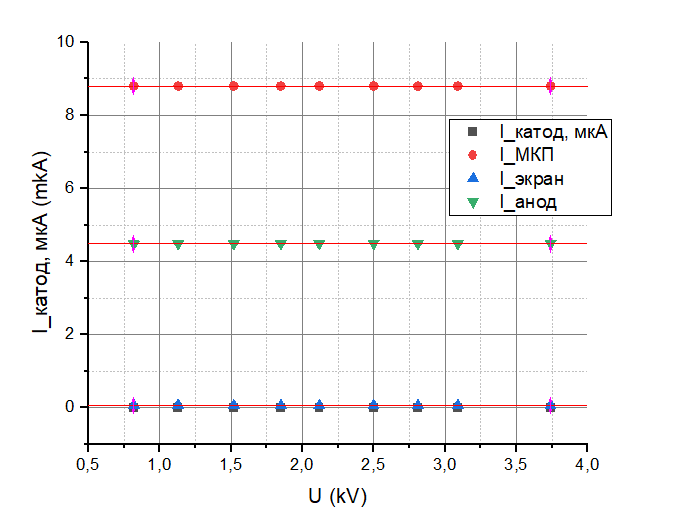
\includegraphics[scale=1]{3}
	\label{graph:ekran}
	\caption{Зависимость токов от напряжения на экране}
	\end{center}
\end{figure}

\newpage


При максимальном напряжении на МКП понижаем напряжение на катоде до минимального уровня, при котором видно изображение. Далее мы понижаем напряжение на  МКП попутно повышая напряжение на катоде, стараясь сохранять постоянный уровень яркости изображения. Полученные значения напряжений занесем в Таблицу $\ref{table:voltages}$

\begin{table}[h]
\begin{center}
\caption{Зависимость напряжения на МКП от напряжения на катоде}
\label{table:voltages}
\begin{tabular}{|c|c|c|c|c|c|c|c|c|c|c|}
\hline
\textbf{$U_{МКП}$}, кВ   & {2,01} & {1,83} & {1,73} & {1,6} & 1,53 & 1,45 & 1,4  & 1,38 & 1,34 & 1,34 \\ \hline
\textbf{$U_{катод}$}, кВ & 1,84          & 2             & 2,23          & 2,4          & 2,8  & 3,04 & 3,25 & 3,52 & 4    & 4,26 \\ \hline
\end{tabular}
\end{center}
\end{table}

По данным Таблицы $\ref{table:voltages}$ построим график зависимости напряжения на катоде от напряжения на МКП

\begin{figure}[h!]
	\begin{center}
	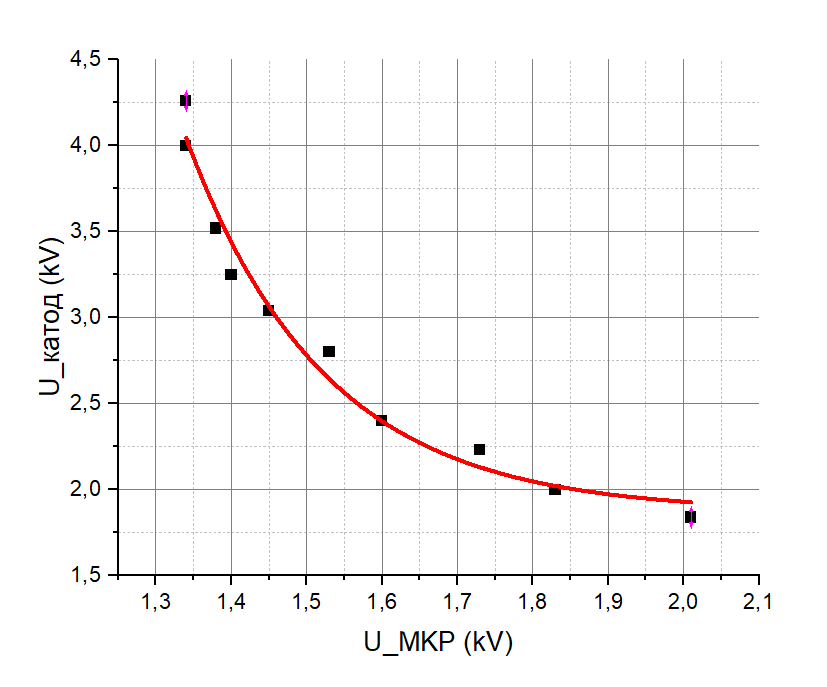
\includegraphics[scale=0.8]{last}
	\label{graph:voltages}
	\caption{Зависимость напряжения на катоде от напряжения на МКП}
	\end{center}
\end{figure}

\section*{Выводы}

1.Исходя из полученных данных, можно сделать вывод о том что ток экрана и катода остаются равными нулю при изменении напряжений на катоде, МКП, экране. \\
2.Токи на МКП и аноде остаются постоянными при изменении напряжений на экране и катоде. \\
3.Зависимость тока катода и анода от напряжения на МКП хорошо аппроксимируются линейной функцией. 




\end{document}